\section{Results}
Table~\ref{tab:a3bench_results} summarizes model performance on A$^3$Bench. We report both overall accuracy, computed as the question-count-weighted average, and category average, computed as the unweighted mean across Basic, Compound, and Detailed questions. Overall, current MLLMs perform poorly on the benchmark: most models achieve below 50\% accuracy, and even the best-performing model reaches only 46.96\% overall accuracy and 44.30\% category average. These results indicate that aggressive action and association remains challenging for state-of-the-art systems. In particular, current MLLMs struggle when evaluation moves beyond coarse aggression recognition and requires identifying who is involved, what action occurs, and how participants are related.

\begin{table}[t]
\small
\centering
\caption{\textbf{Benchmarking models on A$^3$Bench.} Reported metric is accuracy (\%) for Basic Questions, Compound Questions, Detailed Questions, Overall, and Average. \textbf{Best} and \underline{second-best} performance are highlighted.
}
\label{tab:a3bench_results}
\resizebox{\textwidth}{!}{
\begin{tabular}{l | c c c c c}
\toprule
\textbf{Model}
& \textbf{Basic} \textuparrow
& \textbf{Compound} \textuparrow
& \textbf{Detailed} \textuparrow
& \textbf{Overall} \textuparrow
& \textbf{Average} \textuparrow \\
\midrule
gemma-4-26B-A4B-it \cite{gemma4} & 49.07 & 39.65 & 30.86 & 42.72 & 39.86 \\
GPT5.1 \AB{need cite} & 45.63 & 39.17 & 33.32 & 41.30 & 39.37 \\
InternVideo2.5-8B \cite{internvideo2_5} & 48.07 & 39.34 & 21.51 & 40.70 & 36.31 \\
InternVL2.5-8B \cite{internvideo2_5} & \textbf{52.61} & \underline{45.01} & 26.75 & \underline{45.77} & 41.46 \\
InternVL3-9B \cite{internvl3} & 50.05 & 39.06 & 28.22 & 42.55 & 39.11 \\
InternVL3.5-8B \cite{internvl3_5} & 48.34 & 37.03 & 28.75 & 41.06 & 38.04 \\
LLaVA-Video-7B-Qwen2 \cite{llavavideo} & 19.58 & 19.34 & 13.11 & 18.50 & 17.34 \\
Ovis2.5-9B \cite{ovis2_5} & 50.62 & 37.99 & 33.09 & 43.16 & 40.57 \\
Qwen2.5-VL-7B-Instruct \cite{qwen-vl2_5} & 41.87 & 37.15 & 23.73 & 37.30 & 34.25 \\
Qwen3-VL-8B-Instruct \cite{qwen3vl} & 51.07 & \textbf{46.65} & \underline{35.19} & \textbf{46.96} & \textbf{44.30} \\
VideoLLaMA3-7B \cite{videollama3} & 49.65 & 30.86 & 21.41 & 38.22 & 33.97 \\
Qwen2.5-VL-72B-Instruct \cite{qwen-vl2_5} & 45.73 & 39.47 & 26.91 & 40.53 & 37.37 \\
\midrule
Qwen3-VL-8B-Thinking \cite{qwen3vl} & 44.59 & 36.41 & 30.77 & 39.37 & 37.26 \\
InternVL3.5-8B CoT prompt & \underline{51.53} & 38.92 & 33.13 & 43.94 & 41.19 \\
InternVL3.5-8B DoT \cite{navigatinghallucinations} & 49.64 & 40.31 & \textbf{40.90} & 44.77 & \underline{43.62} \\
\bottomrule
\end{tabular}
}
\end{table}

\subsection{Analysis}
\textbf{Performance degrades as aggression understanding becomes more compositional.}
Models achieve an average accuracy of 47.74\% on \textit{Basic} questions, but performance drops to 38.82\% on \textit{Compound} questions and further to 29.58\% on \textit{Detailed} questions. This monotonic decline shows that current MLLMs do not simply fail at rare aggression labels; they fail progressively as the task requires role-action binding. Models can sometimes identify isolated visual cues, such as an action category, a salient participant, or a single role, but struggle once these cues must be composed into a structured interaction. \textit{Compound} questions expose failures in binding two attributes, such as linking the correct action to the correct aggressor or victim. \textit{Detailed} questions further require the full aggressor-action-victim structure, or who did what to whom. The sharp drop on these questions indicates failures in directionality, role assignment, and person-action binding.

Model-level trends show that the compositional drop is not uniform across systems. VideoLLaMA3-7B exhibits the steepest collapse, suggesting strong reliance on single-attribute cues. Qwen2.5-VL-7B-Instruct shows a small Basic-to-Compound drop but a much larger Compound-to-Detailed drop, indicating that pairwise association does not transfer to full aggressor-action-victim reasoning. Ovis2.5-9B and Ovis2.5-9B-Thinking show the reverse pattern, with larger early drops and smaller later drops, suggesting that role-action binding is their main bottleneck. Qwen3-VL-8B-Instruct achieves the strongest Compound performance but still degrades on Detailed questions, while LLaVA-Video-7B-Qwen2 remains weak across all tiers. The DoT variant is a notable exception, with Detailed accuracy slightly exceeding Compound accuracy, suggesting that structured reasoning may help complete interaction-level understanding.

%\AB{Model-wise, the drop-off rate varies dramatically. VideoLLaMA3-7B has the steepest collapse, suggesting it relies almost entirely on single-frame cues. InternVL2.5-78B degrades most gracefully in absolute terms (60.8\% to 45.8\%, -15pp) but within the InternVL2.5 family, the scale gap widens with complexity: +8.1pp at Basic but +19.0pp at Detailed, showing scale disproportionately helps compositional reasoning. In contrast, Qwen2.5-VL shows only a uniform +3pp gain from 7B to 72B across all tiers. Ovis2.5-9B is notable for holding up relatively well on Detailed (33.1\%) despite middling Basic scores (50.6\%), suggesting a different internal reasoning strategy.}

\begin{figure}[h!]
  \centering
    \centering
    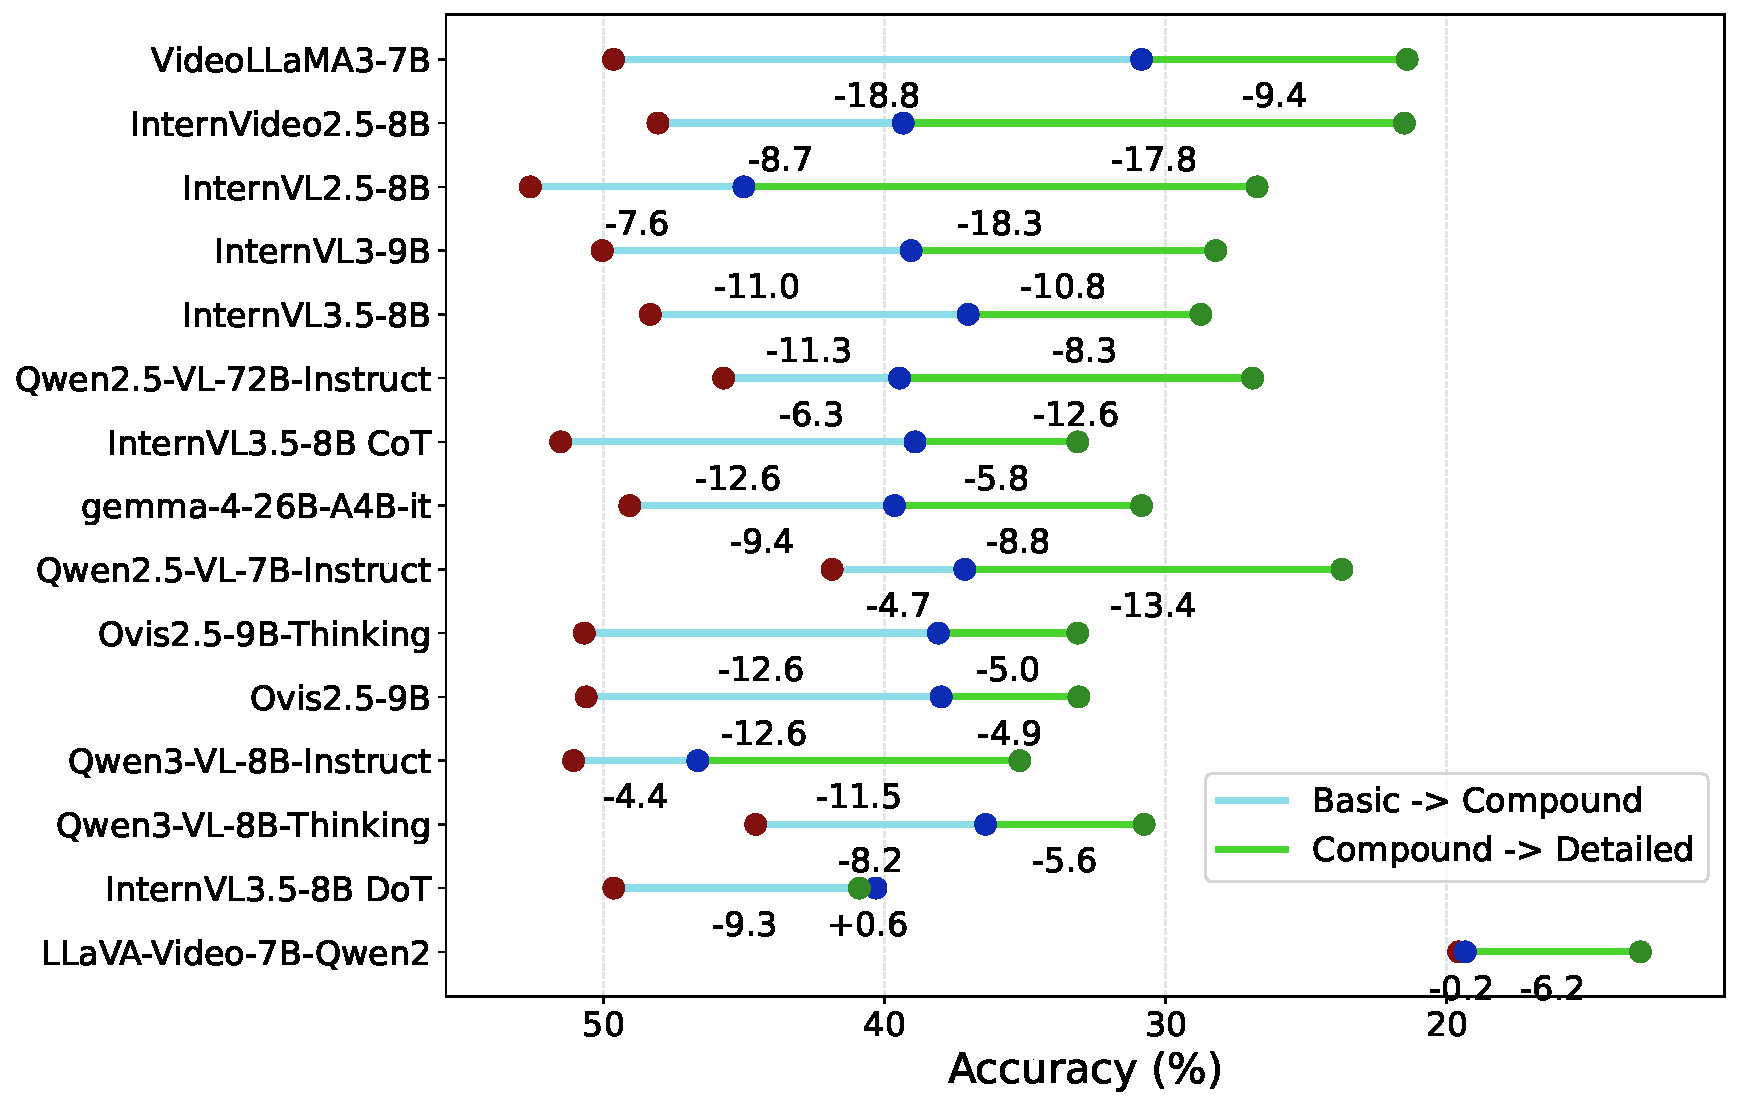
\includegraphics[width=\linewidth]{figures/scores_drop_dumbbell_plot.pdf}
    
  \caption{\textbf{Model wise drop.} \RA{keep or send to supplementary?}
}

  \label{fig:scores_drop_dumbbell_plot.pdf}
\end{figure}

\textbf{Explicit reasoning does not reliably resolve role-action association.}
Reasoning-style variants show limited gains and do not outperform the strongest general-purpose model. Their average overall accuracy remains only 42.83\%, indicating that prompting models to produce intermediate reasoning is not sufficient for reliable aggressive action and association. This suggests that the bottleneck is not only the absence of verbal reasoning, but a deeper weakness in grounding aggressive actions to the correct participants, distinguishing active roles from visible bystanders, and preserving the directionality of the interaction. \RA{Will be much shorter, we are removing ovis thinking}

% \AB{The one exception is InternVL3.5-8B-DoT (Dream of Thoughts), which achieves the flattest compositional curve of any model (49.6\% Basic to 40.9\% Detailed, only -8.7pp drop) and the second-best Detailed score (40.9\%) despite a mediocre Basic score. This is the only reasoning variant that clearly helps on the hardest questions. Qwen3-VL-8B-Thinking actually hurts: it scores 44.6\% Basic vs 51.1\% for non-thinking Qwen3, a 6.5pp regression. Ovis-Thinking is statistically identical to non-thinking Ovis (+0.08pp overall). The pattern suggests that generic ``think step-by-step'' prompting is insufficient -- the reasoning must be structured around the specific decomposition the task requires (as DoT does with its scene graph approach).}

%% 



\begin{figure}[t]
  \centering

  \begin{minipage}[t]{0.34\linewidth}
    \vspace{0pt}
    \centering

    \subcaptionbox{Action vs. role correctness\label{fig:action_vs_agg_or_victim_cm}}{
      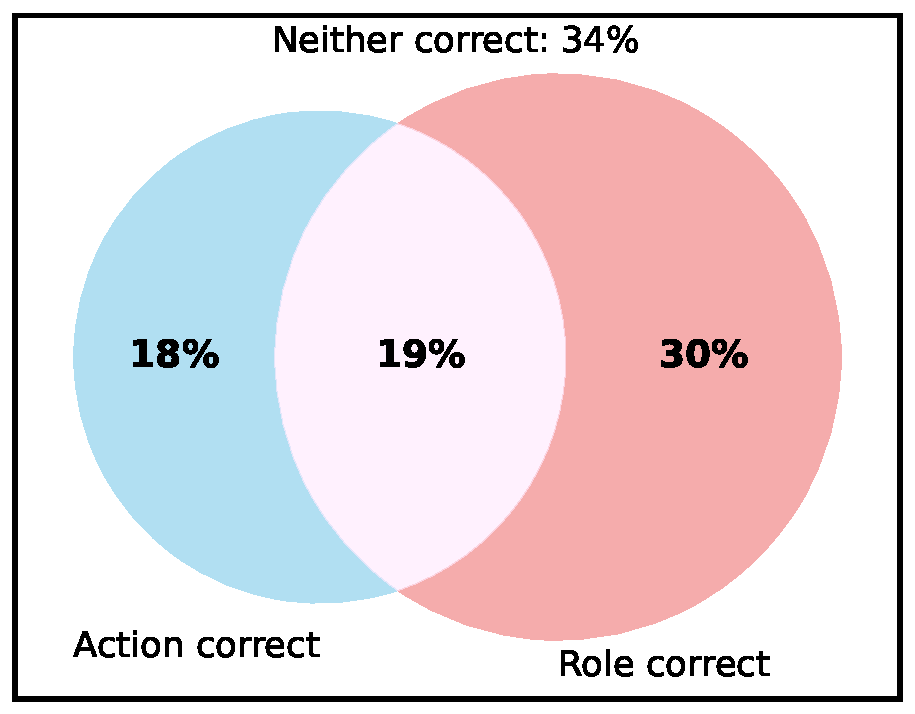
\includegraphics[width=\linewidth]{figures/calculate_action_vs_agg_or_victim_venn.pdf}
    }

    \vspace{1em}

    \subcaptionbox{Aggressor vs. victim correctness\label{fig:victim_vs_aggressor_cm}}{
      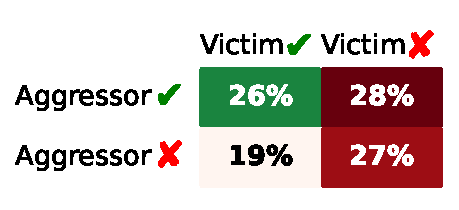
\includegraphics[width=\linewidth]{figures/calculate_victim_vs_aggressor_cm.pdf}
    }
  \end{minipage}
  \hfill
  \begin{minipage}[t]{0.64\linewidth}
    \vspace{0pt}
    \centering

    \subcaptionbox{Role identification confusion matrix\label{fig:role_confusion_matrix}}{
      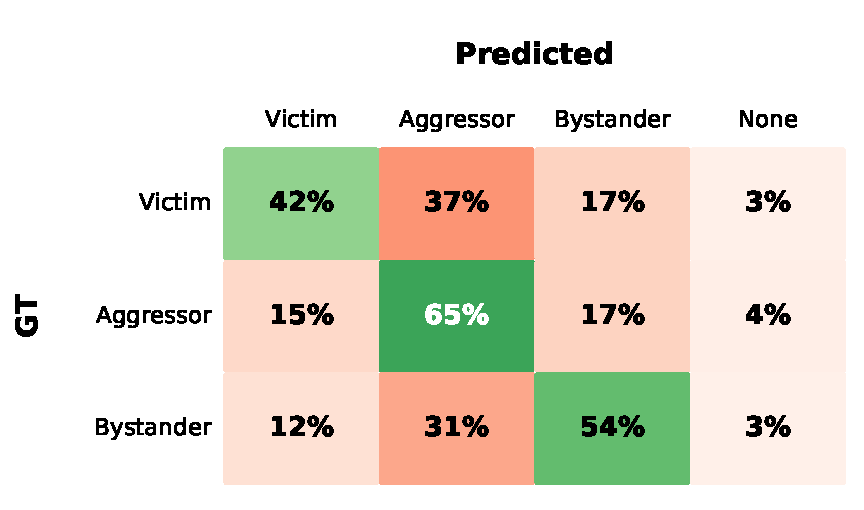
\includegraphics[width=\linewidth]{figures/role_confusion_matrix.pdf}
    }
  \end{minipage}

  \caption{\textbf{Error analysis of action and role association.}
We analyze model failures on basic questions by decomposing predictions across primary aggressive action recognition, aggressor/victim identification, and role classification. The results indicate that current MLLMs struggle not only to recognize aggressive actions, but also to assign the correct roles to the people involved.
\YSR{this is for which model? the left plots are also confusion matrix? its not clear... how about bar chart? not clear what we are showing here... make it easier for the reader..}
}
  \label{fig:error_analysis}
\end{figure}


\noindent\textbf{\textit{Models often identify participants without recognizing the correct aggressive action.}}
To understand whether errors arise from recognizing the aggressive behavior or identifying the relevant participants, we analyze videos that include both a primary action question and at least one aggressor or victim identification question. Figure~\ref{fig:error_analysis}(a) reports results averaged across models. Models are more likely to identify the correct aggressor or victim while failing to recognize the correct action (30\%) than to recognize the correct action while failing to identify the relevant role (18\%). This indicates that models may localize socially salient people in the scene, but still fail to distinguish the fine-grained aggressive action being performed. Thus, even when participant grounding partially succeeds, current MLLMs often lack reliable aggression understanding. 
\RA{discuss model wise with diagram from supplementary}

\YSR{seems like all this analysis is on average scores across all models... it will be good to also have something similar for each model... we might find some interesting pattern for each models? most of it will go in supp, but we can choose what to show here... just average across models might not be good... think about how to present it... visuals will be more dense..}

% \AB{Per-model heatmap (supplementary Figure~\ref{fig:supp_heatmap}) shows this pattern is not uniform. InternVL2.5-78B achieves 64.4\% on Aggressor ID and 54.9\% on Primary Action -- a smaller gap than most models, suggesting scale helps action recognition catch up to role detection. LLaVA-Video-7B is an outlier: it scores below 20\% on both action and role questions, so the action-vs-role decomposition does not apply -- it fails at both. VideoLLaMA3-7B has a uniquely lopsided profile: 53.9\% on Aggressor ID but only 22.6\% on Action+Aggressor compound, indicating it can sometimes locate the right person but cannot bind an action to them.}



\noindent\textbf{\textit{Models are biased toward assigning the aggressor role.}}
Figures~\ref{fig:error_analysis}(b,c) show a consistent role-grounding failure: models tend to over-assign the aggressor role when identifying participants in aggressive interactions. In Figure~\ref{fig:error_analysis}(b), when only one of the two roles is correct, models more often identify the aggressor while misidentifying the victim (28\%) than identify the victim while misidentifying the aggressor (19\%). Figure~\ref{fig:error_analysis}(c) makes this bias more explicit: a substantial fraction of ground-truth victims (37\%) and bystanders (31\%) are incorrectly predicted as aggressors. These errors suggest that models often treat visual involvement, proximity, or saliency as evidence of aggression, rather than reasoning about who initiates the action and who is targeted. As a result, they collapse distinct participant roles into a generic ``involved person'' representation, making victim and bystander grounding unreliable.

\AB{Per-model role confusion matrices (supplementary Figure~\ref{fig:supp_role_confusion}) reveal this asymmetry is extreme in some models: Ovis2.5-9B mislabels 54.3\% of true victims as aggressors, and InternVL3.5-8B reaches 47.7\%. The reverse (aggressor-to-victim) is much lower for these same models (11.0\% and 7.1\% respectively). InternVL2.5-8B shows the opposite bias: it has the worst aggressor-to-victim confusion (30.3\%) but relatively low victim-to-aggressor (17.8\%). This suggests fundamentally different internal attention strategies across architectures -- some models default to ``aggressor'' for any salient person, others distribute confusion more evenly.}

\AB{The confusion matrices make this concrete: across all models, the ``Aggressor'' column dominates predictions regardless of true role. Bystanders are classified as aggressors at rates of 30--45\% for most models (InternVL3.5-8B: 39.5\%, VideoLLaMA3: 36.5\%), meaning models treat any visible person near an altercation as a likely aggressor. LLaVA-Video-7B has a uniquely flat confusion profile -- it distributes predictions almost uniformly across all roles (20--30\% each), indicating it has no strong role prior but also no real understanding.}

\noindent\textbf{\textit{Same-video and role-reversal distractors expose weak visual grounding.}}
Distractor analysis shows that models are especially vulnerable when incorrect options are visually grounded in the same clip or preserve parts of the correct interaction structure. For Basic person-identification questions, same-video role-based distractors are more challenging than cross-video distractors because the incorrect participant is genuinely visible in the video. For Compound and Detailed questions, role-reversal distractors expose failures in directionality: models often select answers that contain the correct people and action but swap the aggressor and victim. Bystander substitutions reveal a related weakness, where models assign active roles to people who are merely present in the scene. In Detailed questions, frequency-inverted distractors further show that models may rely on answer-choice priors rather than visual grounding, selecting options with familiar or frequently co-occurring action-role-person components instead of recovering the full aggressor-action-victim structure.
\RA{Discuss from supplementary with category wise figure}

\AB{Distractor vulnerability heatmap (supplementary Figure~\ref{fig:supp_distractor}) quantifies this: role reversal causes 22--28\% of all errors across every model, confirming it is the single most effective distractor type. The vulnerability profile is strikingly uniform -- even the strongest models show the same proportional weakness to role reversal as weaker models. LLaVA-Video-7B is the one outlier with a distinctly different profile: it is much more susceptible to wrong\_aggressor (7.6\%), wrong\_victim (9.2\%), and bystander\_substitution (8.7\%) than other models (1--5\% each), confirming a broad person-identification failure rather than a directional reasoning deficit.}

\noindent\textbf{\textit{Models over-predict aggression even in non-aggressive clips.}}
We also conduct a free-form social appropriateness evaluation on five relatively strong models from the Ovis, InternVL, and Qwen families~\cite{ovis2_5, internvl2_5, qwen3vl}. Each model is asked to characterize the social appropriateness of the action shown in a video. Models are generally able to identify aggressive or socially inappropriate behavior in the 2,234 aggressive clips. However, on the 449 non-aggressive clips, they frequently still attribute inappropriate or aggressive behavior to the videos, achieving below approximately 60\% accuracy, close to random binary performance. This indicates that current models are sensitive to aggressive cues but also exhibit a strong aggression prior, over-predicting aggression even when no aggressive behavior is present.
\RA{Waiting for model scores from Austin}

\AB{Negation question analysis (supplementary Figure~\ref{fig:supp_trick}) reveals this bias varies enormously by model. InternVL3.5-8B drops 31.9pp on negation questions (47.8\% standard to 15.8\% negation -- nearly chance). InternVL3-9B and InternVL3.5-8B-CoT show similar gaps (31.1pp, 30.2pp), suggesting the InternVL3 family has a particularly strong aggression prior that reasoning prompts do not fix. In contrast, Gemma-4-26B is nearly calibrated (only 2.1pp gap, 45.7\% vs 43.6\%), and LLaVA-Video-7B actually scores slightly better on negation questions (-2.9pp gap), though both its accuracies are low. This per-model variation indicates the aggression prior is architecture-dependent, not an inherent property of the task.}

\noindent\textbf{\textit{Scene context adds another layer of grounding difficulty.}}
We further evaluate whether models can associate aggressive actions with their surrounding scene context using a subset of videos (detailed results in Supplementary) where the environment is clearly identifiable. Models are asked to identify both the action and the environment in which it occurs. Adding this scene-grounding requirement makes the task harder for most models: average accuracy drops from 40.53\% for primary action recognition to 36.69\% for action-environment association. This suggests that models are not only challenged by recognizing aggressive actions, but also by grounding those actions in the correct environmental context. While action recognition can often rely on local motion or appearance cues, action-environment association requires joint reasoning over the behavior and the broader scene.

\AB{Per the question-type heatmap (supplementary Figure~\ref{fig:supp_heatmap}), the Action+Location type averages only 36.3\% across models -- lower than most Compound types. Qwen3-VL-8B is the strongest here (46.7\%), substantially ahead of the next best. This suggests Qwen3's architecture may be better at jointly encoding spatial context with action information, possibly due to its vision encoder design or pretraining data composition.}

\YSR{this looks pretty good... great job... see if some of the above analysis can be shown as visuals/tables/etc., and less verbose... also, do we have any experiments with number of frames as input?}

\begin{comment}
\textbf{Counting}

To isolate whether models struggle with visual counting or role
assignment, we compare performance on two types of counting questions:
\emph{aggregate counts} that ask for the total number of people involved
(``how many aggressors and victims?'') and \emph{role-specific counts}
that require isolating individuals by their role (``how many
aggressors?''). This assessment was performed on the three highest achieving models 
from the benchmark test.

\begin{table}[t]
\centering
\caption{Counting accuracy (\%) on 4-option questions (chance = 25\%).
Aggregate counts require detecting people involved; role-specific counts
require assigning aggressor/victim/bystander roles first.}
\label{tab:counting}
\small
\begin{tabular}{lccc}
\toprule
Question Type & InternVL2.5-8B & Qwen3-8B & InternVL2.5-78B \\
\midrule
\multicolumn{4}{l}{\textit{Aggregate counts}} \\
\quad Aggressor + Victim     & 85.6 & 80.1 & 85.6 \\
\quad Victim + Bystander     & 94.9 & 87.9 & 95.8 \\
\midrule
\multicolumn{4}{l}{\textit{Role-specific counts}} \\
\quad Aggressor only         & 34.7 & 32.1 & 41.8 \\
\quad Victim only            & 52.2 & 52.6 & 64.2 \\
\quad Bystander only         & 26.1 & 29.9 & 17.2 \\
\midrule
Overall                      & 56.0 & 54.2 & 58.4 \\
\bottomrule
\end{tabular}
\end{table}

Models count people reliably (80--96\%) but fail when they must assign
roles first (25--42\% for aggressors and bystanders).
This confirms that role assignment --- not visual counting --- is the
bottleneck, and that counting questions probe the same capability as our
primary benchmark.
\end{comment}

\begin{comment}
We analyze this along three axes (Table~\ref{tab:text_shortcuts}). First, answer-position bias is mild: positions A--D hold the correct answer at 14.7--15.2\% versus 9.0--11.0\% for E--H, against a 12.5\% chance baseline. The elevated rate for early positions is an artifact of role identification questions, which admit only four plausible answer choices (aggressor, victim, bystander, or none) and thus concentrate correct answers in positions A--D. Second, certain negation phrases (e.g., ``no aggressive action is taking place'') appear exclusively as correct answers because they describe non-aggressive clips and cannot serve as plausible distractors elsewhere. 

Left: correct answer position distribution across 12,773 questions (chance = 12.5\%). Right: 
\begin{tabular}{c c c}
\toprule
\textbf{Pos.} & \textbf{Count} & \textbf{\%} \\
\midrule
A & 1,929 & 15.1 \\
B & 1,873 & 14.7 \\
C & 1,945 & 15.2 \\
D & 1,874 & 14.7 \\
E & 1,408 & 11.0 \\
F & 1,342 & 10.5 \\
G & 1,258 & 9.8 \\
H & 1,144 & 9.0 \\
\midrule
\textit{Chance} & & \textit{12.5} \\
\bottomrule
\end{tabular}
\hspace{8pt}

\end{comment}

\begin{comment}
Third, we directly test exploitation by comparing model accuracy when the correct answer is the most vs.\ least frequently occurring text. As shown in Table~\ref{tab:text_shortcuts}, all models achieve near-identical accuracy in both conditions (e.g., 64.3\% vs.\ 64.1\% for InternVL2.5-78B), confirming that performance reflects visual understanding rather than text-frequency pattern matching.

\begin{table}[h!]
\centering
\caption{\textbf{Text-only shortcut analysis.} model accuracy on questions where the correct answer is the most vs.\ least frequent text.}
\label{tab:text_shortcuts}
\scriptsize
\resizebox{0.5\linewidth}{!}{
\begin{tabular}{l c c c}
\toprule
\textbf{Model} & \textbf{Acc.} & \textbf{Most Freq} & \textbf{Least Freq} \\
\midrule
InternVL2.5-78B & 59.3 & 64.3 & 64.1 \\
InternVL2.5-8B & 50.3 & 63.2 & 65.4 \\
Qwen3-VL-8B & 49.9 & 61.6 & 64.5 \\
InternVL3.5-8B & 48.7 & 61.7 & 63.6 \\
Ovis2.5-9B & 48.2 & 60.8 & 65.6 \\
\bottomrule
\end{tabular}
}
\end{table}
\end{comment}